\documentclass[10pt,a4paper]{article}
\usepackage[utf8]{inputenc}
\usepackage{amsmath}
\usepackage{amsfonts}
\usepackage{amssymb}
\usepackage{german}
\usepackage{fancyhdr}
\usepackage{graphicx}
\usepackage{geometry}
\usepackage{color}
\usepackage[usenames,dvipsnames]{xcolor}
\usepackage{DejaVuSans}
\usepackage[T1]{fontenc}
\renewcommand*{\familydefault}{\sfdefault}
\geometry{verbose,a4paper,tmargin=35mm,bmargin=35mm,lmargin=25mm,rmargin=25mm}
\author{Dominik Heeb, Fabian Keller}
\title{Projektplan Bachelorarbeit}
\pagestyle{fancy}
\fancyhead{}
\fancyhead[L]{Projektplan - Verkehrsmodell-Fallstudien-Editor}
\fancyhead[R]{Domink Heeb, Fabian Keller}
\fancyfoot{}
\fancyfoot[R]{Seite \thepage}
\begin{document}
\begin{titlepage}
	\begin{Huge}
		\begin{center}
				Projektplan \\Verkehrsmodell-Fallstudien-Editor\\[2.0cm]
		\end{center}
	\end{Huge}
	
	\begin{center}
		\begin{Large}
				von Dominik Heeb, Fabian Keller\\[1.0cm]
		\end{Large}
		\begin{large}
				Betreuer: Prof. Dr. Luc Bläser
		\end{large}
	\end{center}
\end{titlepage}

\newpage
\tableofcontents 
\newpage

\section{Management Abläufe}
\begin{flushleft}
	Diese Bachelorarbeit wird im Rahmen des Bachelor Studiums an der HSR durchgeführt welches bei erfolgreichem Abschluss mit 12 ECTS Punkten gewertet wird. Ein ECTS Punkt entspricht einem ungefähren Zeitaufwand von 25 bis 30 Stunden. Somit wird von jedem Teammitglied ein Zeitaufwand von ca. 300 bis 360 Stunden erwartet.
\end{flushleft}

\subsection{Zeitliche Planung}
	\begin{flushleft}
Der zeitliche Projektplan zeigt eine grobe zeitliche Übersicht über die gesamte Bachelorarbeit mit den einzelnen Iterationen und Meilensteinen.
	\end{flushleft}
	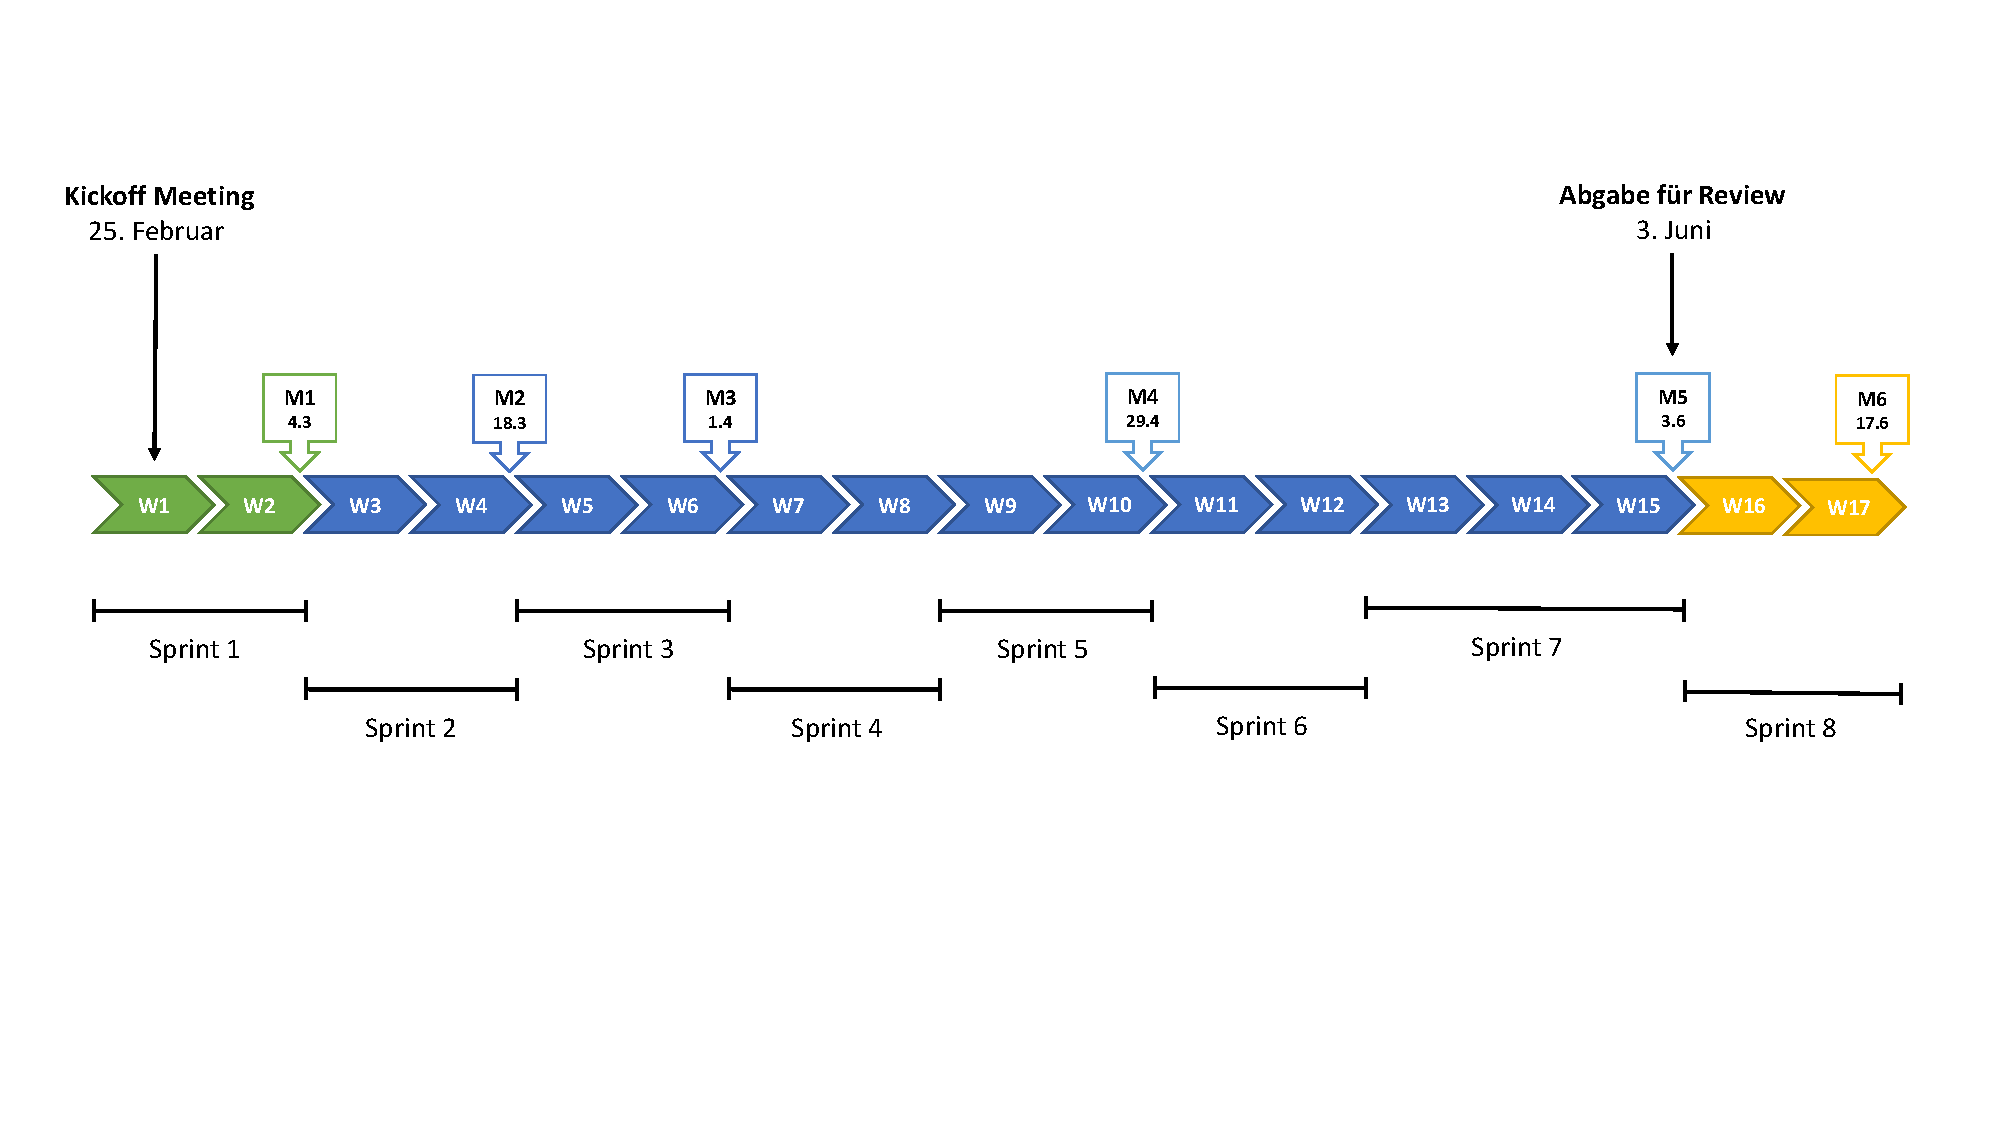
\includegraphics[width=17cm,height=7cm,trim=10mm 40mm 0mm 20mm, clip]{pictures/Meilensteinplan.pdf}

\subsection{Meilensteine}
\begin{flushleft}
	Die einzelnen Meilensteine, die bereits in der zeitlichen Planung ersichtlich sind, beinhalten folgende Ziele:
\end{flushleft}
\begin{tabular}{cl}
	\textcolor{Orange}{\textbf{M1:}} & Projektplanung erstellt (Projektplan, )\\[0.2cm]
	\textcolor{Orange}{\textbf{M2:}} & Funktionale und nicht funktionale Anforderungen, Konzepte um Verkehrsdaten\\[0.1cm]
		& effizient und übersichtlich darzustellen, Kommunikationskonzept zwischen Frontend\\[0.2cm]
		& und Backend, Design der Software-Architektur, Prototyp\\[0.2cm]
	\textcolor{NavyBlue}{\textbf{M3:}} & Verkehrsdaten auf Frontend darstellen\\[0.2cm]
	\textcolor{NavyBlue}{\textbf{M4:}} & Definierte Änderungen an Verkehrsdaten können vorgenommen werden\\[0.2cm]
	\textcolor{Dandelion}{\textbf{M5:}} & Präsentation der Bachelorarbeit, Abgabe Bericht\\
\end{tabular}
\subsection{Besprechungen}
\begin{flushleft}
	Die Besprechung findet jede Woche am Donnerstag im Raum 1.167 um 14:00 Uhr statt. In dieser Besprechung wird der aktuelle Status der Bachelorarbeit besprochen, offene Fragen geklärt und das weitere Vorgehen besprochen.\\
Das Projektteam erstellt vor jeder Besprechung eine Traktandenliste und führt ein Protokoll. Dieses Protokoll wird anschliessend an den Betreuer und die Auftraggeber gesendet.
\end{flushleft}
\subsection{Risiken}
\begin{flushleft}
\begin{tabular}{l l l}
Risiko & Wahrscheinlichkeit & Potential\\
\hline
Datenmenge zu gross & mittel & mittel\\
Backend Implementierung zu aufwändig & klein & mittel\\
\end{tabular}\\[0.2cm]
\subsubsection*{Datenmenge zu gross}
Dieses Risiko enthält die Gefahr das durch zu grosse Datenmengen die Client-Side Implementierung des Editor zu aufwändig wird. Die Folge daraus wäre das der Editor nicht zufriedenstellend entwickelt werden kann. Eine Massnahme um die Wahrscheinlichkeit des Eintretens klein zu halten ist es, von Anfang an die Menge der Daten in die Implementierung und Konzeptionierung einfliessen zu lassen.\\[0.2cm]
\subsubsection*{Backend Implementierung zu aufwändig}
Die Konzeptionierung des Verkehrsmodell-Editor behandelt hauptsächlich die Frontend Entwicklung. Wenn der Backend zu komplex wird, bleibt zu wenig Zeit den Frontend ansprechend zu entwickeln. Die Massnahme ist, den Backend auf das Wesentliche zu beschränken und die Entwicklung des Frontend in den Vordergrund zu stellen. Funktionen für den Backend sollten wenn sie zu viel Zeit brauchen vereinfacht werden.\\

\end{flushleft}
\newpage
\section{Vorgehen}
\subsection{Projektmanagement}
\subsubsection{Aufbau}
\begin{itemize}
	\item Elaboration: 
	\item Construction: 
	\item Transition: 
\end{itemize}
\subsubsection{Tools}
Für das Projektmanagement werden folgende Tools verwendet:
\begin{itemize}
\item JIRA: für die Planung und Verwaltung der Arbeitspakete.
\item GitHub: Der Code und die Dokumentation werden über Github Repositories verwaltet
\item CI Server (JetBrains TeamCity): Mittels eines CI Server wird die Qualität und Lauffähigkeit des Codes geprüft
\item TexMaker: Latex Editor für die Dokumentation
\item IntelliJ IDEA 15: IDE für Java Entwicklung
\end{itemize}
\subsection{Entwicklung}
\subsubsection{Vorgehen}
Die Entwicklung der Bachelorarbeit wird als Agiles Softwareprojekt aufgebaut.
\subsubsection{Unit Testing}
\subsubsection{Code Reviews}
Code Reviews und Pair Programming sind Methoden um die Qualität des Codes innerhalb des Teams hoch zu halten
\subsubsection{Code Analyse}
\subsubsection{Code Style Guidelines}
\end{document}